% ══════════════════════════════════════════════════════════════════════════
\section{Introducción}

Colombia se ubica cerca del ecuador terrestre, entre aproximadamente $4^\circ$\,S y
$12^\circ$\,N de latitud, lo que hace que la duración del día varíe muy poco a lo largo
del año y, por tanto, no experimentamos las estaciones climáticas típicas de las
latitudes medias y altas.
Sin embargo, el fenómeno astronómico que origina las estaciones —el movimiento aparente
del Sol a lo largo de la \textbf{eclíptica}— sí puede detectarse desde Colombia si se
miden con precisión las horas de salida y puesta del astro \citep{CarrollOstlie2017}.

Esta práctica analiza la variación anual de las horas de luz solar en cinco ciudades
distribuidas entre latitudes $+60{,}17^\circ$\,N y $-53{,}16^\circ$\,S.
La comparación de las efemérides en ciudades de distintos hemisferios permite evidenciar,
en toda su magnitud, el efecto que la inclinación axial de la Tierra
($\varepsilon \approx 23{,}44^\circ$) produce sobre los ritmos de iluminación diurna a
lo largo del globo \citep{Meeus1998}.

% ══════════════════════════════════════════════════════════════════════════
\section{Objetivos}

\subsection{Objetivo general}

Comprender el movimiento anual aparente del Sol y su relación con las estaciones del
año, mediante el análisis de la variación de las horas de salida y puesta del Sol en
ciudades de distintas latitudes durante el año 2026.

\subsection{Objetivos específicos}

\begin{itemize}
  \item Identificar las diferencias en la duración del día y la noche en distintas
        latitudes, en los hemisferios norte y sur.
  \item Obtener las efemérides del Sol (horas de salida y puesta) para cinco ciudades
        mediante \texttt{astroplan} \citep{Morris2018} y validarlas con el servicio
        \textit{JPL Horizons} \citep{Giorgini1996}.
  \item Analizar y comparar cómo varían las efemérides en función de la latitud y la
        época del año.
  \item Explicar las causas astronómicas detrás de las variaciones observadas.
\end{itemize}

% ══════════════════════════════════════════════════════════════════════════
\section{Marco teórico}

\subsection{Movimiento aparente del Sol y la eclíptica}

Desde la Tierra, el Sol parece desplazarse lentamente por la esfera celeste a lo largo
de un círculo máximo llamado \textbf{eclíptica}, completando una vuelta en
${\approx}365{,}25$ días (año trópico).
Este movimiento es, en realidad, el reflejo del traslado de la Tierra alrededor del Sol,
pero se manifiesta como un cambio continuo en la \textbf{declinación solar}
($\delta_\odot$): el ángulo que forma el Sol con el ecuador celeste
\citep{CarrollOstlie2017}.

La declinación solar varía entre $-23{,}44^\circ$ (solsticio de diciembre) y
$+23{,}44^\circ$ (solsticio de junio), y es cero en los dos equinoccios:

\begin{table}[H]
  \centering
  \caption{Fechas aproximadas de los principales eventos solares en 2026 y la
           declinación solar correspondiente
           \citep{CarrollOstlie2017, Meeus1998}.}
  \label{tab:eventos}
  \begin{tabular}{lll}
    \toprule
    \textbf{Evento} & \textbf{Fecha aprox.\ 2026} & \textbf{Declinación $\delta_\odot$} \\
    \midrule
    Equinoccio de Marzo (vernal)  & 20 de marzo      & $0^\circ$       \\
    Solsticio de Junio            & 21 de junio      & $+23{,}44^\circ$ \\
    Equinoccio de Septiembre      & 22 de septiembre & $0^\circ$       \\
    Solsticio de Diciembre        & 21 de diciembre  & $-23{,}44^\circ$ \\
    \bottomrule
  \end{tabular}
\end{table}

\subsection{Ángulo horario de salida/puesta del Sol y duración del día}

El Sol sale y se oculta cuando su altura sobre el horizonte es cero.
Para un observador en latitud $\varphi$, esto ocurre cuando el ángulo horario~$H$
satisface \citep{Meeus1998}:

\begin{equation}
  \cos(H_0) = -\tan(\varphi)\,\tan(\delta_\odot).
  \label{eq:H0}
\end{equation}

El ángulo $H_0$ obtenido corresponde al semiarco diurno; la duración del día en horas
es:

\begin{equation}
  T_{\text{día}} = \frac{2\,H_0}{15^\circ/\text{h}},
  \label{eq:Tdia}
\end{equation}

donde $H_0$ se expresa en grados.
En la práctica se aplica una corrección de $-0{,}833^\circ$ al horizonte geométrico para
contabilizar la refracción atmosférica estándar y el semidiámetro angular del Sol
\citep{Meeus1998}.

\subsection{Casos extremos}

\begin{itemize}
  \item \textbf{Latitud $> 66{,}56^\circ$\,(N o S):}  En verano la noche no llega
        (Sol de medianoche) y en invierno el Sol no sale (noche polar). Helsinki
        ($\varphi \approx +60{,}17^\circ$) se acerca a este régimen y experimenta
        días de invierno de apenas ${\sim}6$\,h y noches de verano casi inexistentes.
  \item \textbf{Ecuador ($\varphi \approx 0^\circ$):} La ecuación~(\ref{eq:H0}) da
        $H_0 \approx 90^\circ$ todo el año, es decir, $T_{\text{día}} \approx 12$\,h
        sin variación apreciable.
  \item \textbf{Equinoccios ($\delta_\odot = 0^\circ$):} Para cualquier latitud,
        la ecuación~(\ref{eq:H0}) da $H_0 = 90^\circ$ y el día dura exactamente $12$\,h
        (descontando la corrección de refracción).
\end{itemize}

% ══════════════════════════════════════════════════════════════════════════
\section{Metodología}

\subsection{Ciudades y coordenadas geográficas}

Se seleccionaron cinco ciudades de acuerdo con las instrucciones de la actividad
(Tabla~\ref{tab:ciudades}).
Las coordenadas se verificaron con Google Maps \citep{GoogleMaps2026} y los institutos
cartográficos nacionales correspondientes; las altitudes provienen de la misión
\textit{Shuttle Radar Topography Mission} (SRTM).

\begin{table}[H]
  \centering
  \caption{Coordenadas geográficas de las cinco ciudades de estudio
           \citep{GoogleMaps2026}.}
  \label{tab:ciudades}
  \begin{tabular}{llcccc}
    \toprule
    \textbf{Ciudad} & \textbf{País} & \textbf{$\varphi$ (°)} &
    \textbf{$\lambda$ (°)} & \textbf{Alt.\ (m)} & \textbf{Hemisferio} \\
    \midrule
    Helsinki              & Finlandia & $+60{,}17$ & $+24{,}94$ &    0 & Norte \\
    Aguascalientes        & México    & $+21{,}89$ & $-102{,}29$ & 1888 & Norte \\
    UdeA (Medellín)       & Colombia  & $+6{,}27$  & $-75{,}57$  & 1530 & Norte \\
    Río de Janeiro        & Brasil    & $-22{,}91$ & $-43{,}17$  &   10 & Sur   \\
    Punta Arenas          & Chile     & $-53{,}16$ & $-70{,}92$  &    8 & Sur   \\
    \bottomrule
  \end{tabular}
\end{table}

\subsection{Herramientas computacionales}

Se utilizó el paquete \texttt{astroplan} \citep{Morris2018}, una librería afiliada a
\texttt{astropy} que implementa el cálculo riguroso de eventos astronómicos basado en
datos del IERS y en la corrección de horizonte de $-0{,}833^\circ$.
Las funciones \texttt{sun\_rise\_time()} y \texttt{sun\_set\_time()},
del objeto \texttt{Observer}, calculan para cada fecha el amanecer previo
y el atardecer siguiente al mediodía local.

Los resultados se validaron comparando las horas calculadas con el servicio
\textit{JPL Horizons} \citep{Giorgini1996} para Helsinki el día del solsticio de junio
de 2026 (21 de junio).
\texttt{astroplan} reportó la salida del Sol a las 00:53 UTC, mientras que
\textit{JPL Horizons} indicó las 01:05 UTC, una diferencia de 12 minutos atribuible a
distintos modelos de refracción atmosférica e interpolación numérica.

\subsection{Fechas de observación}

Se calcularon las efemérides para 19 fechas distribuidas a lo largo del año 2026, con
un intervalo de 20 días entre fechas consecutivas, comenzando el 1 de enero de 2026.

% ══════════════════════════════════════════════════════════════════════════
\section{Resultados}

\subsection{Horas de salida y puesta del Sol}

La Tabla~\ref{tab:salida_puesta} presenta las horas de salida y puesta del Sol en cada
ciudad para las 19 fechas de observación.
Las horas se expresan en la zona horaria \textbf{local} de cada ciudad, en formato
HH:MM, tal como indica la guía de la práctica.

\begin{table}[H]
  \centering
  \caption{Horas de salida y puesta del Sol (salida -- puesta, hora local) en las cinco
           ciudades de estudio durante 2026.
           Fuente: \texttt{astroplan} \citep{Morris2018}.}
  \label{tab:salida_puesta}
  {\scriptsize
  \begin{tabular}{lccccc}
    \toprule
    \textbf{Fecha} &
    \textbf{Helsinki} &
    \textbf{Aguascalientes} &
    \textbf{UdeA (Medellín)} &
    \textbf{Río de Janeiro} &
    \textbf{Punta Arenas} \\
    \midrule
    01/01/2026 & 09:24 -- 15:23 & 07:28 -- 18:17 & 06:12 -- 17:59 & 05:10 -- 18:41 & 05:21 -- 22:12 \\
    21/01/2026 & 08:58 -- 16:04 & 07:29 -- 18:31 & 06:19 -- 18:08 & 05:24 -- 18:42 & 05:52 -- 21:56 \\
    10/02/2026 & 08:12 -- 16:57 & 07:23 -- 18:43 & 06:19 -- 18:13 & 05:38 -- 18:35 & 06:32 -- 21:22 \\
    02/03/2026 & 07:16 -- 17:49 & 07:09 -- 18:53 & 06:14 -- 18:14 & 05:49 -- 18:20 & 07:11 -- 20:38 \\
    22/03/2026 & 06:16 -- 18:39 & 06:51 -- 19:00 & 06:05 -- 18:12 & 05:57 -- 18:01 & 07:48 -- 19:50 \\
    11/04/2026 & 06:15 -- 20:28 & 06:32 -- 19:07 & 05:56 -- 18:10 & 06:04 -- 17:42 & 08:24 -- 19:03 \\
    01/05/2026 & 05:17 -- 21:18 & 06:17 -- 19:15 & 05:49 -- 18:09 & 06:12 -- 17:26 & 08:59 -- 18:21 \\
    21/05/2026 & 04:28 -- 22:07 & 06:07 -- 19:23 & 05:46 -- 18:11 & 06:21 -- 17:17 & 09:31 -- 17:48 \\
    10/06/2026 & 03:57 -- 22:42 & 06:05 -- 19:32 & 05:47 -- 18:16 & 06:29 -- 17:14 & 09:54 -- 17:31 \\
    30/06/2026 & 03:59 -- 22:47 & 06:09 -- 19:36 & 05:51 -- 18:20 & 06:34 -- 17:18 & 09:59 -- 17:35 \\
    20/07/2026 & 04:32 -- 22:19 & 06:16 -- 19:34 & 05:55 -- 18:21 & 06:31 -- 17:26 & 09:43 -- 17:56 \\
    09/08/2026 & 05:18 -- 21:31 & 06:24 -- 19:24 & 05:57 -- 18:18 & 06:21 -- 17:34 & 09:11 -- 18:27 \\
    29/08/2026 & 06:07 -- 20:33 & 06:31 -- 19:08 & 05:55 -- 18:10 & 06:05 -- 17:41 & 08:29 -- 19:00 \\
    18/09/2026 & 06:54 -- 19:32 & 06:36 -- 18:49 & 05:52 -- 18:00 & 05:46 -- 17:47 & 07:41 -- 19:34 \\
    08/10/2026 & 07:42 -- 18:31 & 06:42 -- 18:30 & 05:49 -- 17:50 & 05:26 -- 17:54 & 06:53 -- 20:09 \\
    28/10/2026 & 07:32 -- 16:34 & 06:50 -- 18:14 & 05:48 -- 17:43 & 05:10 -- 18:03 & 06:08 -- 20:47 \\
    17/11/2026 & 08:24 -- 15:45 & 07:02 -- 18:05 & 05:52 -- 17:42 & 05:00 -- 18:15 & 05:32 -- 21:26 \\
    07/12/2026 & 09:07 -- 15:15 & 07:15 -- 18:06 & 06:00 -- 17:46 & 04:59 -- 18:28 & 05:12 -- 21:58 \\
    27/12/2026 & 09:25 -- 15:17 & 07:26 -- 18:14 & 06:10 -- 17:56 & 05:07 -- 18:39 & 05:16 -- 22:12 \\
    \bottomrule
  \end{tabular}
  }
\end{table}
\newpage
La Figura~\ref{fig:salida_puesta} representa la evolución de las horas de salida y
puesta del Sol a lo largo del año.
En Helsinki se aprecia la mayor variación: la salida del Sol oscila entre las
09:25 (diciembre) y las 03:57 (junio), y la puesta entre las 15:15 y las 22:47.
En la Universidad de Antioquia, ambas horas permanecen casi constantes a lo largo del
año.

\begin{figure}[H]
  \centering
  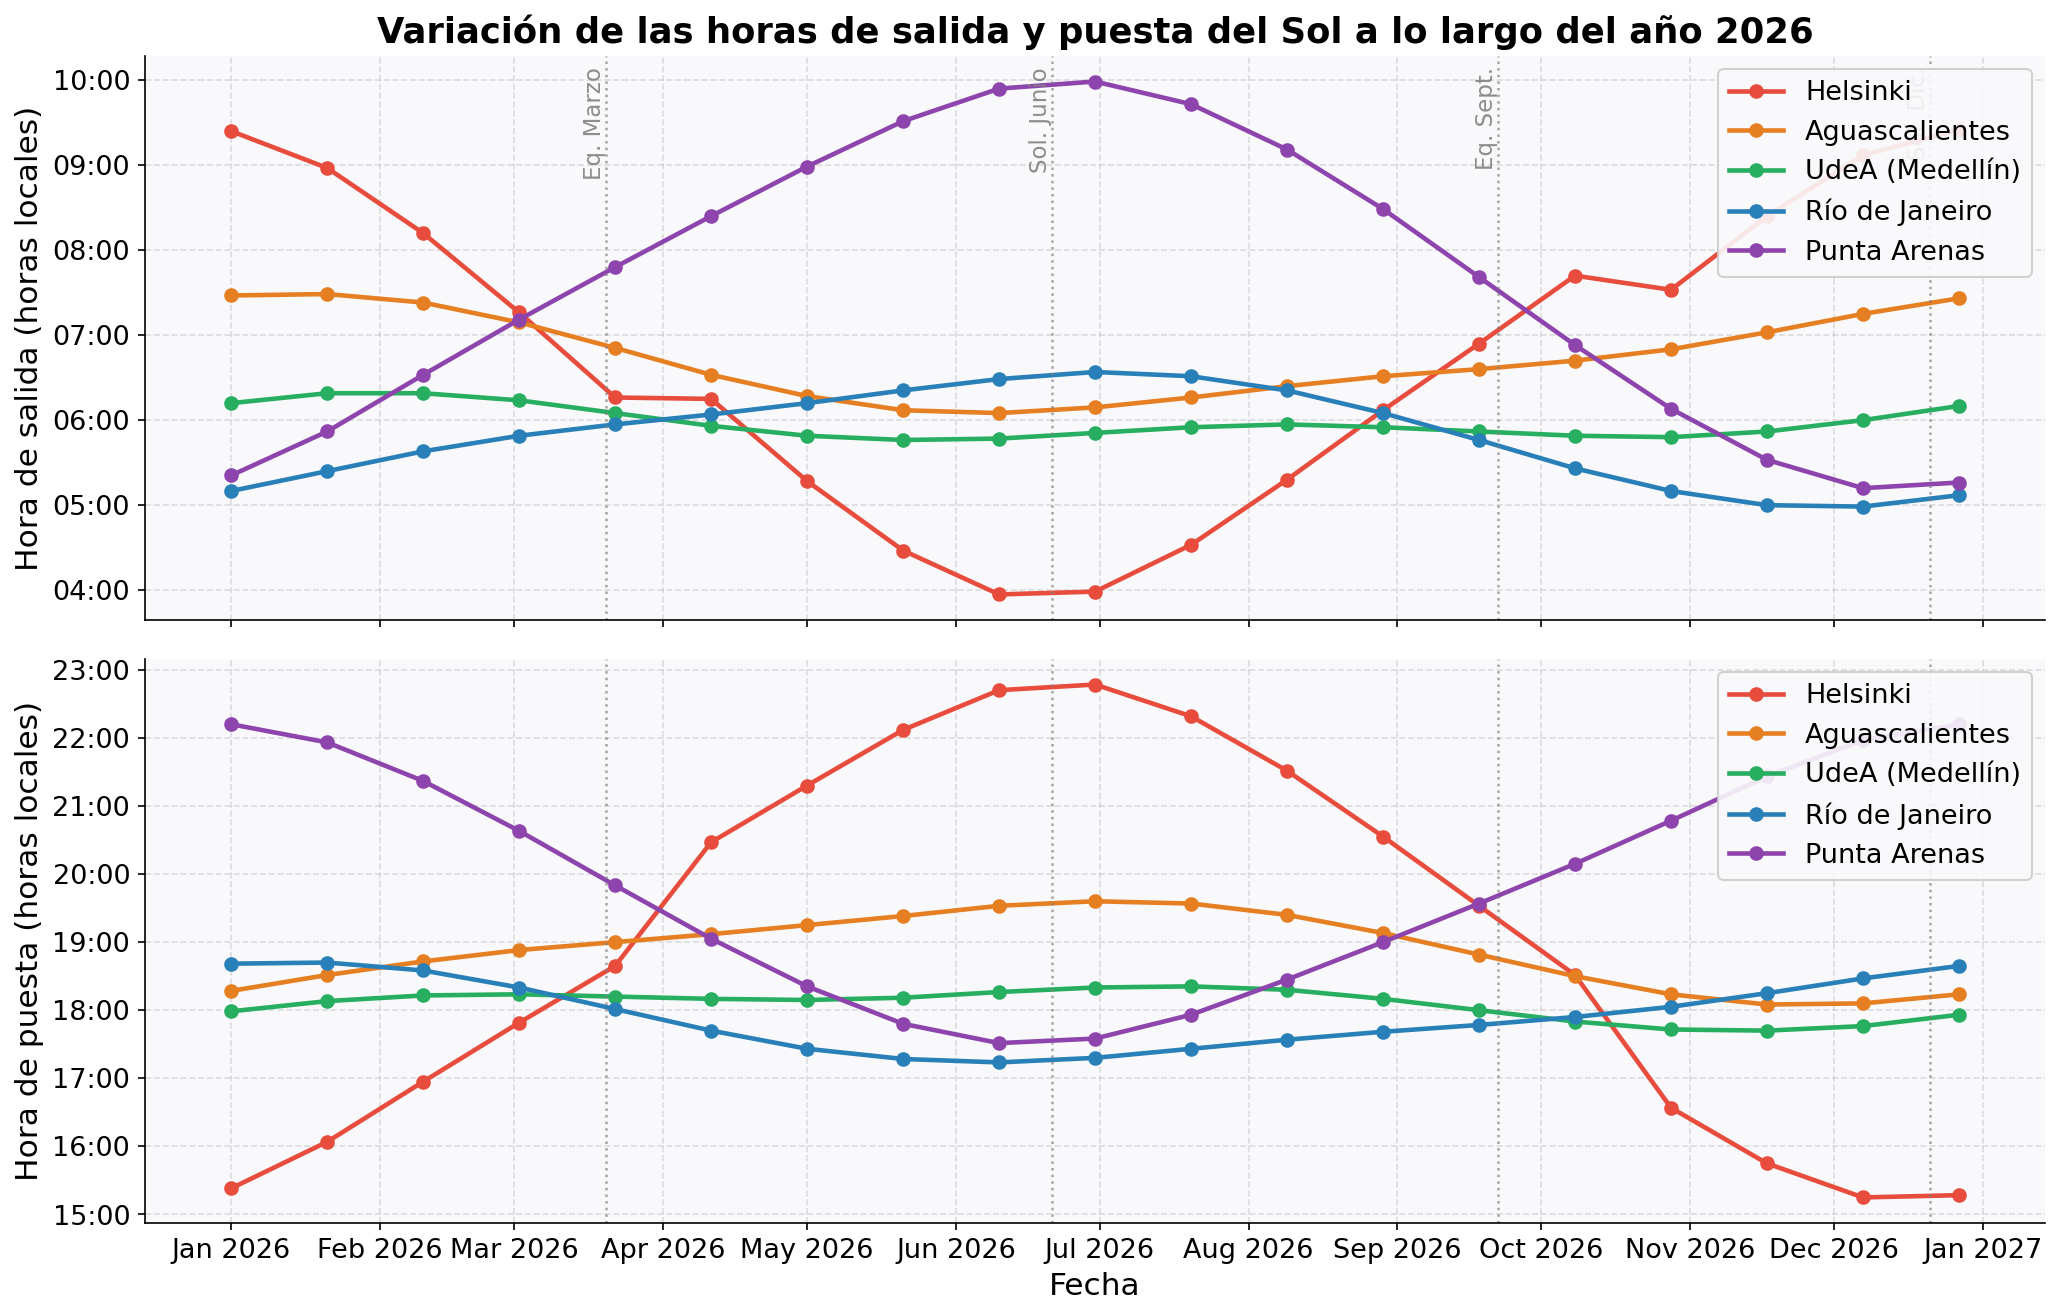
\includegraphics[width=0.95\textwidth]{imagenes/fig1_salida_puesta.png}
  \caption[Horas de salida y puesta del Sol en las cinco ciudades]{Horas de salida
           (\textit{panel superior}) y puesta (\textit{panel inferior}) del Sol
           en las cinco ciudades a lo largo de 2026.
           Fuente: \texttt{astroplan} \citep{Morris2018}.}
  \label{fig:salida_puesta}
\end{figure}
\newpage
\subsection{Duración del día}

La Tabla~\ref{tab:duracion} presenta la duración del día para cada ciudad y fecha.

\begin{table}[H]
  \centering
  \caption{Duración del día solar (horas y minutos de luz) en las cinco ciudades durante
           2026.
           Fuente: \texttt{astroplan} \citep{Morris2018}.}
  \label{tab:duracion}
  {\scriptsize
  \begin{tabular}{lccccc}
    \toprule
    \textbf{Fecha} &
    \textbf{Helsinki} &
    \textbf{Aguascalientes} &
    \textbf{UdeA (Medellín)} &
    \textbf{Río de Janeiro} &
    \textbf{Punta Arenas} \\
    \midrule
    01/01/2026 & 05\,h\,59\,min & 10\,h\,50\,min & 11\,h\,46\,min & 13\,h\,31\,min & 16\,h\,50\,min \\
    21/01/2026 & 07\,h\,06\,min & 11\,h\,01\,min & 11\,h\,49\,min & 13\,h\,18\,min & 16\,h\,04\,min \\
    10/02/2026 & 08\,h\,44\,min & 11\,h\,21\,min & 11\,h\,54\,min & 12\,h\,56\,min & 14\,h\,50\,min \\
    02/03/2026 & 10\,h\,33\,min & 11\,h\,44\,min & 12\,h\,01\,min & 12\,h\,31\,min & 13\,h\,27\,min \\
    22/03/2026 & 12\,h\,23\,min & 12\,h\,10\,min & 12\,h\,07\,min & 12\,h\,04\,min & 12\,h\,02\,min \\
    11/04/2026 & 14\,h\,13\,min & 12\,h\,35\,min & 12\,h\,14\,min & 11\,h\,38\,min & 10\,h\,39\,min \\
    01/05/2026 & 16\,h\,01\,min & 12\,h\,58\,min & 12\,h\,20\,min & 11\,h\,15\,min & 09\,h\,22\,min \\
    21/05/2026 & 17\,h\,39\,min & 13\,h\,16\,min & 12\,h\,26\,min & 10\,h\,56\,min & 08\,h\,17\,min \\
    10/06/2026 & 18\,h\,45\,min & 13\,h\,27\,min & 12\,h\,29\,min & 10\,h\,45\,min & 07\,h\,38\,min \\
    30/06/2026 & 18\,h\,49\,min & 13\,h\,27\,min & 12\,h\,29\,min & 10\,h\,45\,min & 07\,h\,36\,min \\
    20/07/2026 & 17\,h\,47\,min & 13\,h\,17\,min & 12\,h\,26\,min & 10\,h\,55\,min & 08\,h\,13\,min \\
    09/08/2026 & 16\,h\,12\,min & 12\,h\,59\,min & 12\,h\,21\,min & 11\,h\,13\,min & 09\,h\,16\,min \\
    29/08/2026 & 14\,h\,26\,min & 12\,h\,37\,min & 12\,h\,15\,min & 11\,h\,36\,min & 10\,h\,32\,min \\
    18/09/2026 & 12\,h\,38\,min & 12\,h\,12\,min & 12\,h\,08\,min & 12\,h\,01\,min & 11\,h\,53\,min \\
    08/10/2026 & 10\,h\,49\,min & 11\,h\,47\,min & 12\,h\,01\,min & 12\,h\,28\,min & 13\,h\,16\,min \\
    28/10/2026 & 09\,h\,02\,min & 11\,h\,24\,min & 11\,h\,55\,min & 12\,h\,53\,min & 14\,h\,39\,min \\
    17/11/2026 & 07\,h\,22\,min & 11\,h\,04\,min & 11\,h\,50\,min & 13\,h\,15\,min & 15\,h\,54\,min \\
    07/12/2026 & 06\,h\,08\,min & 10\,h\,51\,min & 11\,h\,46\,min & 13\,h\,29\,min & 16\,h\,46\,min \\
    27/12/2026 & 05\,h\,52\,min & 10\,h\,49\,min & 11\,h\,46\,min & 13\,h\,32\,min & 16\,h\,56\,min \\
    \bottomrule
  \end{tabular}
  }
\end{table}

La Figura~\ref{fig:duracion} ilustra la evolución de la duración del día a lo largo del
año para las cinco ciudades.

\begin{figure}[H]
  \centering
  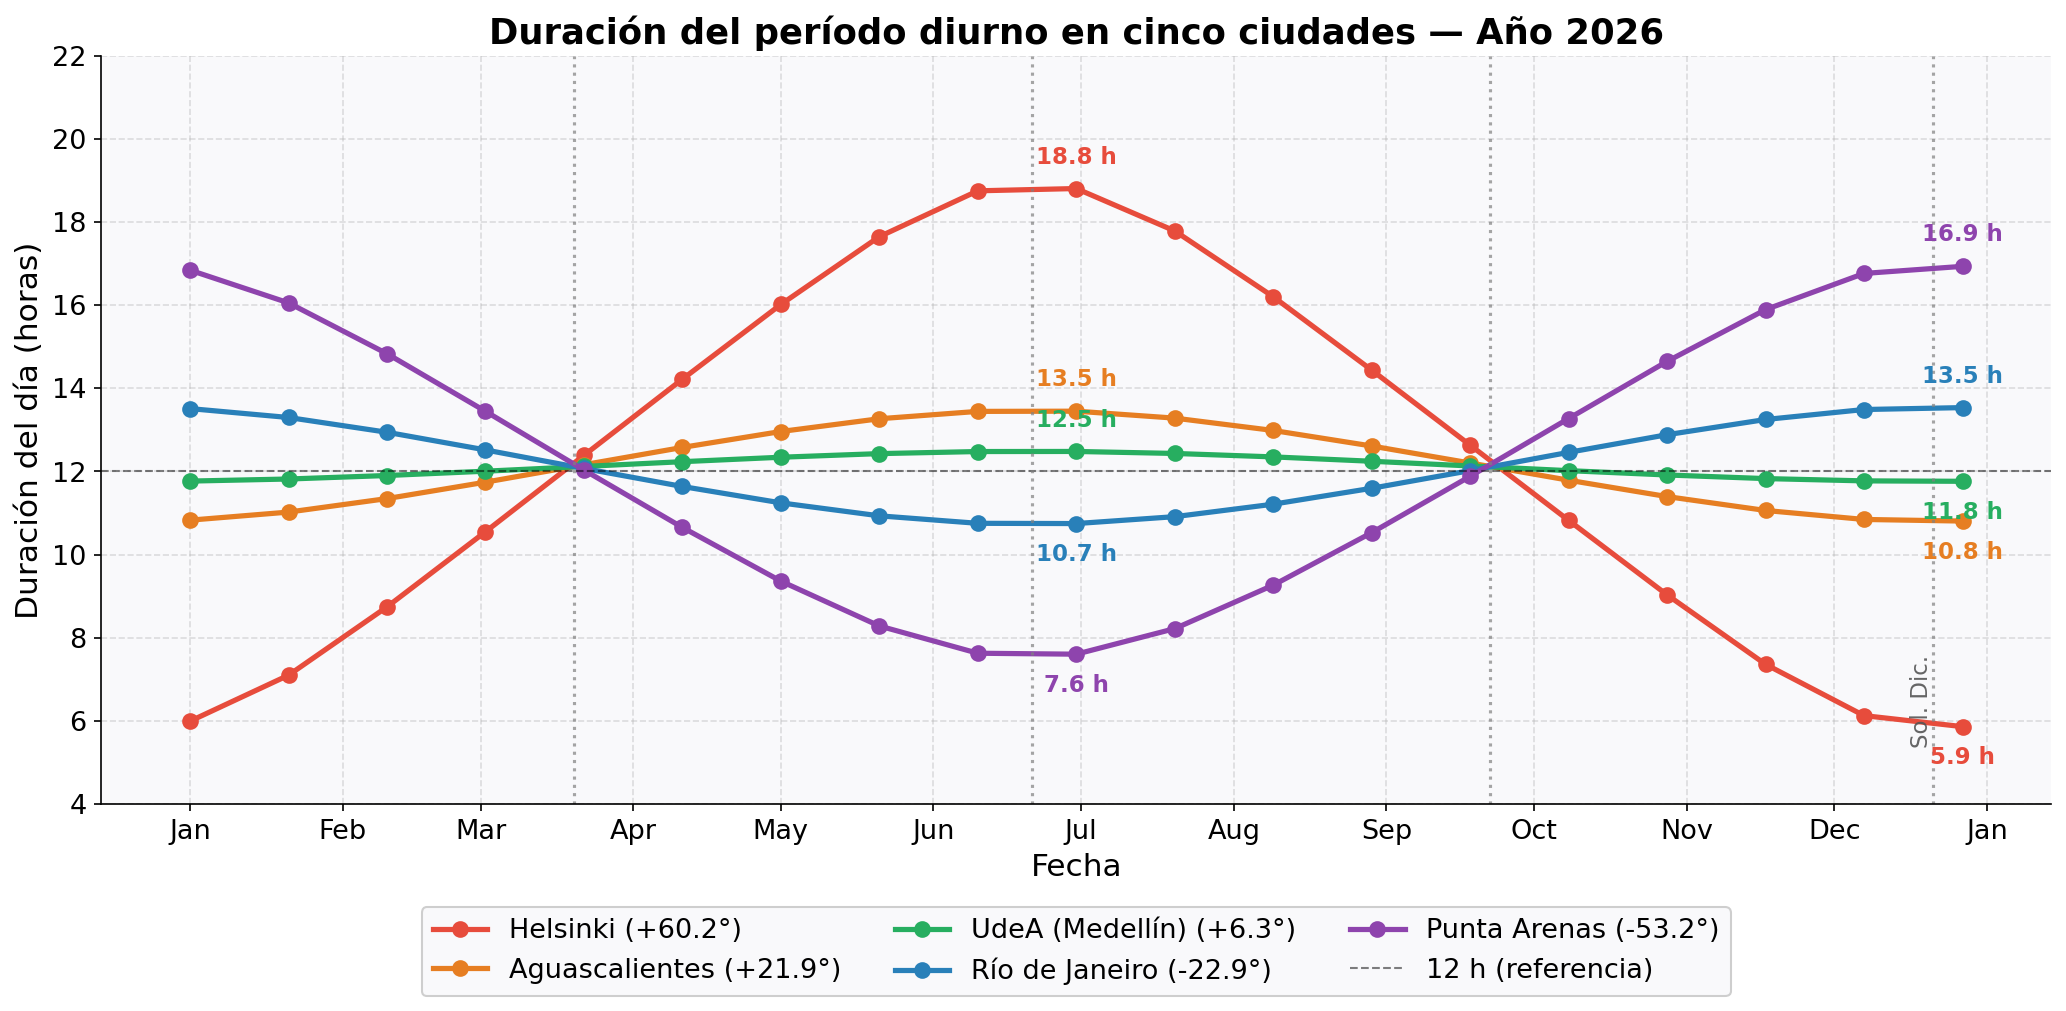
\includegraphics[width=0.95\textwidth]{imagenes/fig2_duracion_dia.png}
  \caption[Duración del día en las cinco ciudades a lo largo de 2026]{Duración del día
           solar en las cinco ciudades a lo largo de 2026.
           Los valores mínimos y máximos de cada ciudad aparecen anotados sobre la
           curva correspondiente.
           Fuente: \texttt{astroplan} \citep{Morris2018}.}
  \label{fig:duracion}
\end{figure}

\subsection{Altitud solar al mediodía}

La Figura~\ref{fig:altitud} muestra la altitud máxima del Sol (al pasar por el meridiano
local) a lo largo del año.
Esta variable mide el ángulo que forma el Sol con el horizonte al mediodía solar y
está directamente relacionada con la intensidad de la radiación que recibe cada lugar:
a mayor altitud, mayor energía por unidad de área.

\begin{figure}[H]
  \centering
  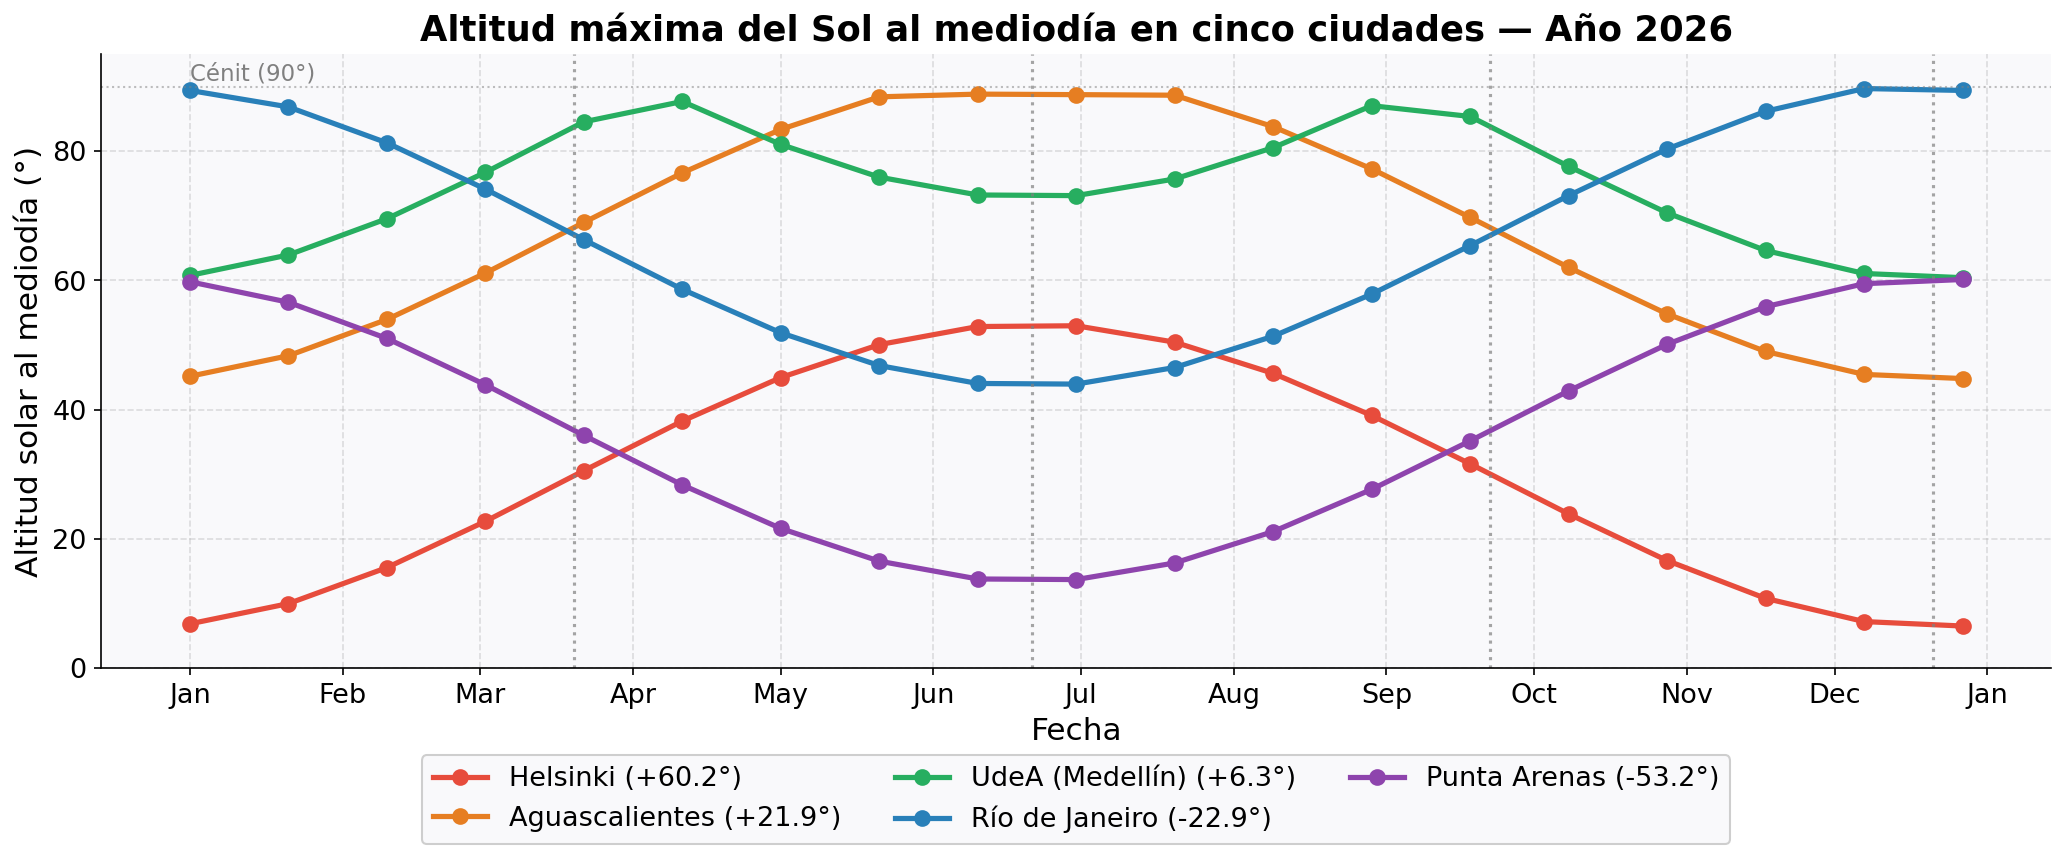
\includegraphics[width=0.95\textwidth]{imagenes/fig3_altitud_mediodia.png}
  \caption[Altitud solar al mediodía en las cinco ciudades]{Altitud solar al mediodía
           (al cruzar el meridiano local) en las cinco ciudades durante 2026.
           Fuente: \texttt{astroplan} \citep{Morris2018}.}
  \label{fig:altitud}
\end{figure}

\subsection{Variabilidad anual de la duración del día}

La Figura~\ref{fig:variabilidad} resume la dispersión de la duración del día en cada
ciudad mediante un diagrama de caja (\textit{boxplot}) y el rango de variación
anual.

\begin{figure}[H]
  \centering
  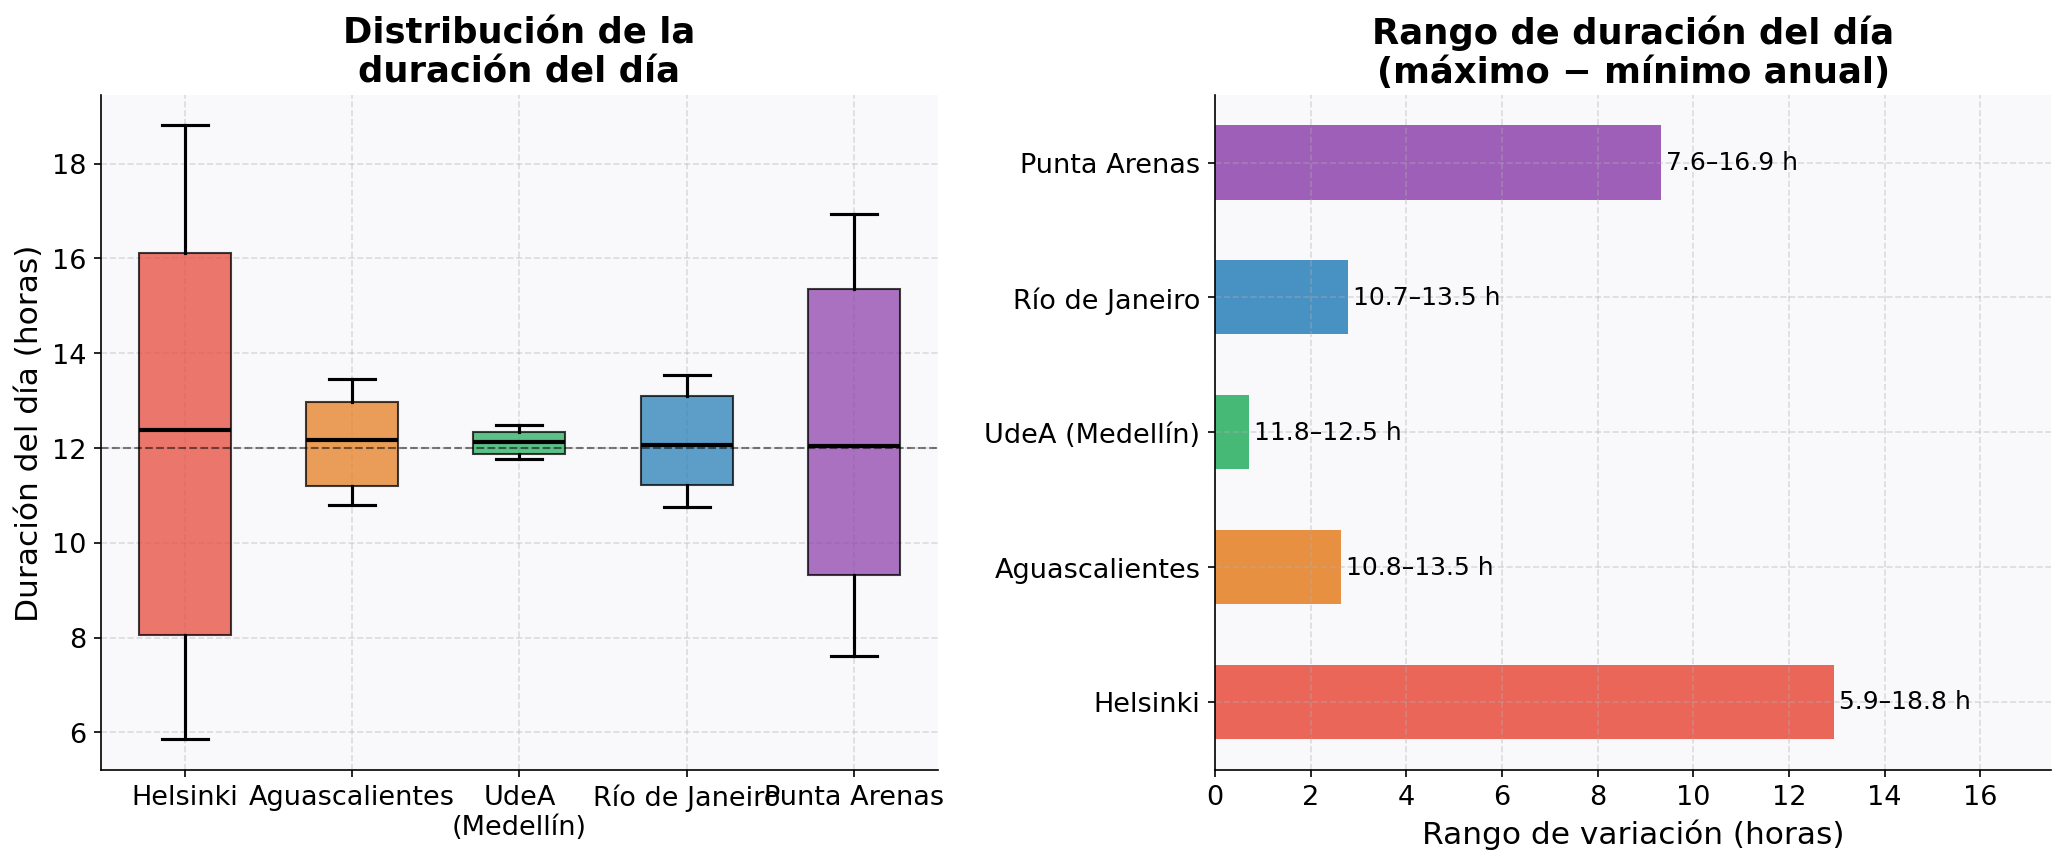
\includegraphics[width=0.95\textwidth]{imagenes/fig4_variabilidad.png}
  \caption[Variabilidad anual de la duración del día]{Variabilidad anual de la duración
           del día solar.
           \textit{Izquierda:} diagrama de caja por ciudad.
           \textit{Derecha:} rango de variación anual (máximo menos mínimo).
           Fuente: \texttt{astroplan} \citep{Morris2018}.}
  \label{fig:variabilidad}
\end{figure}

La Figura~\ref{fig:heatmap} presenta un mapa de calor que muestra la duración del día
organizada por ciudad (de norte a sur) y por fecha, permitiendo visualizar de
manera compacta el comportamiento antisimétrico entre hemisferios.

\begin{figure}[H]
  \centering
  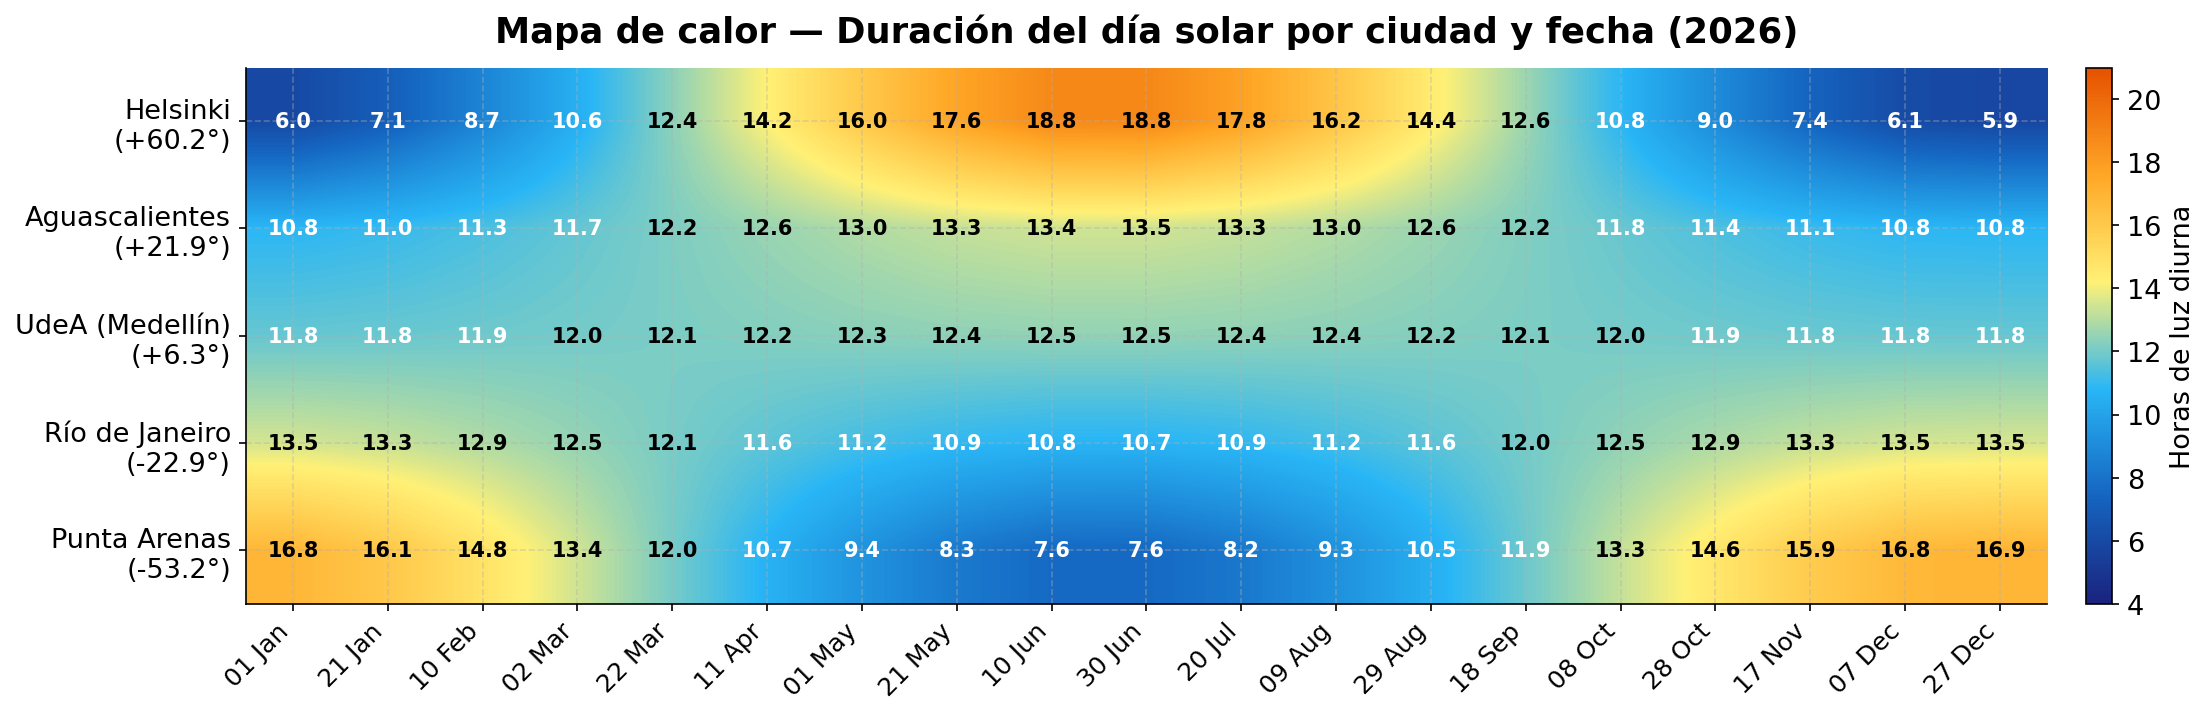
\includegraphics[width=0.95\textwidth]{imagenes/fig5_heatmap.png}
  \caption[Mapa de calor de la duración del día]{Mapa de calor de la duración del día
           solar para las cinco ciudades (de norte a sur, de arriba a abajo) a lo largo
           de 2026.
           Los colores más oscuros (azul) representan noches largas y los más claros
           (amarillo-naranja) representan días largos.
           Fuente: \texttt{astroplan} \citep{Morris2018}.}
  \label{fig:heatmap}
\end{figure}

% ══════════════════════════════════════════════════════════════════════════
\section{Discusión}

\subsection{Comportamiento antisimétrico entre hemisferios}

La comparación entre Helsinki ($\varphi = +60{,}17^\circ$) y Punta Arenas
($\varphi = -53{,}16^\circ$) muestra el comportamiento más contrastante.
Cuando Helsinki alcanza su día más largo (18\,h\,49\,min, en torno al 30 de junio,
solsticio de junio), Punta Arenas registra su día más corto (7\,h\,36\,min);
el patrón se invierte en diciembre: Helsinki mínimo de 5\,h\,52\,min frente al máximo
de Punta Arenas de 16\,h\,56\,min.

Este comportamiento antisimétrico es la consecuencia directa de la
\textbf{inclinación axial de 23{,}44°} de la Tierra \citep{CarrollOstlie2017}:
el eje de rotación terrestre apunta siempre hacia el mismo lugar de la esfera celeste
(cerca de Polaris), de modo que en junio el Polo Norte está inclinado \emph{hacia} el
Sol (verano boreal $=$ invierno austral) y en diciembre lo está el Polo Sur.

\subsection{Latitudes tropicales}

La \textbf{Universidad de Antioquia} ($\varphi \approx +6{,}27^\circ$) presenta una
variación anual de apenas $\approx 43$\,min entre el día más corto (11\,h\,46\,min) y
el más largo (12\,h\,29\,min): un cambio perfectamente observable si se presta atención,
pero que en la vida cotidiana pasa casi desapercibido \citep{IDEAM2014}.
Esto confirma que en Colombia \emph{sí} existe un ciclo diurno anual, aunque muy
atenuado comparado con las latitudes medias.

\textbf{Aguascalientes} ($\varphi = +21{,}89^\circ$) muestra una variación de
$\approx 2$\,h\,38\,min, notablemente mayor que la de Medellín pero mucho menor que la
de Helsinki.
Esto ilustra que la variación de la duración del día aumenta con la latitud de manera
no lineal, conforme a la ecuación~(\ref{eq:H0}).

\subsection{Convergencia en los equinoccios}

Cerca de las fechas de los equinoccios (22 de marzo y 18 de septiembre de 2026,
Tabla~\ref{tab:eventos}), todas las ciudades convergen a una duración de día cercana
a 12\,h (Tablas~\ref{tab:salida_puesta} y \ref{tab:duracion}).
Esto es consistente con la predicción analítica: cuando $\delta_\odot = 0^\circ$,
la ecuación~(\ref{eq:H0}) da $H_0 = 90^\circ$ y $T_{\text{día}} = 12$\,h para cualquier
latitud.
Las pequeñas desviaciones observadas respecto a este valor teórico (del orden de unos
pocos minutos) se deben a la corrección de $-0{,}833^\circ$ por refracción atmosférica y
semidiámetro solar \citep{Meeus1998}.

\subsection{Las estaciones del año: causa astronómica}

Las estaciones del año \emph{no} se deben a la variación en la distancia Tierra-Sol
(la Tierra está más cerca del Sol en enero, en el perihelio, que en julio).
Se deben exclusivamente a la \textbf{inclinación del eje} terrestre, que determina:

\begin{enumerate}
  \item La \textit{duración del día}, que regula las horas de insolación directa
        \citep{CarrollOstlie2017}.
  \item El \textit{ángulo de incidencia} de los rayos solares: a mayor altitud del Sol,
        mayor es la intensidad por unidad de área (Figura~\ref{fig:altitud}).
\end{enumerate}

Ambos efectos combinados producen el exceso de calor en verano y el déficit en invierno
en las latitudes medias y altas.

% ══════════════════════════════════════════════════════════════════════════
\section{Conclusiones}

\begin{enumerate}

  \item Las horas de salida y puesta del Sol varían notablemente con la latitud.
        Helsinki ($\varphi = +60{,}17^\circ$) experimenta un rango de
        $\approx 13$\,h en la duración del día a lo largo del año, mientras que la
        Universidad de Antioquia ($\varphi = +6{,}27^\circ$) muestra una variación de
        apenas $\approx 43$\,min.

  \item El comportamiento de Helsinki y Punta Arenas es perfectamente antisimétrico:
        cuando uno alcanza su máximo de horas de luz, el otro registra su mínimo.
        Esta oposición de fase entre hemisferios es consecuencia directa de la
        inclinación axial de la Tierra \citep{CarrollOstlie2017}.

  \item Cerca de los equinoccios, todas las ciudades —independientemente de su
        latitud— convergen a una duración del día de $\approx 12$\,h, en plena
        concordancia con la predicción de la ecuación~(\ref{eq:H0}).

  \item Las estaciones del año son causadas por la inclinación axial de la Tierra
        ($\varepsilon \approx 23{,}44^\circ$), no por la variación de la distancia
        Tierra-Sol.
        Esta inclinación regula simultáneamente la duración del día y el ángulo de
        incidencia solar, produciendo los contrastes estacionales de temperatura en las
        latitudes medias y altas \citep{CarrollOstlie2017, Meeus1998}.

  \item Las efemérides calculadas con \texttt{astroplan} \citep{Morris2018} son
        consistentes con los datos del servicio \textit{JPL Horizons}
        \citep{Giorgini1996} dentro de una diferencia de ${\approx}12$\,min para el
        caso de prueba analizado (Helsinki, solsticio de junio de 2026), lo que
        confirma la validez de la metodología empleada.

\end{enumerate}
